In this page the admin can browse for users and ban them.
The user can either:
\begin{itemize}
    \item Browse users by username: writing in the input field positioned above the user list and by clicking the "Search" button
    \item Switch between the two kind of users: by clicking the button which is either "See professors" or "See students" the admin can switch the user type in which his searches are performed
    \item ban a user: once he found the user that he want, he can ban it clicking on the button with his name
    \item browse the returned list: once he searched for a specific username, he can go through the results clicking on the buttons positioned at the bottom of the page
\end{itemize}
\begin{figure}[H]
    \centering
    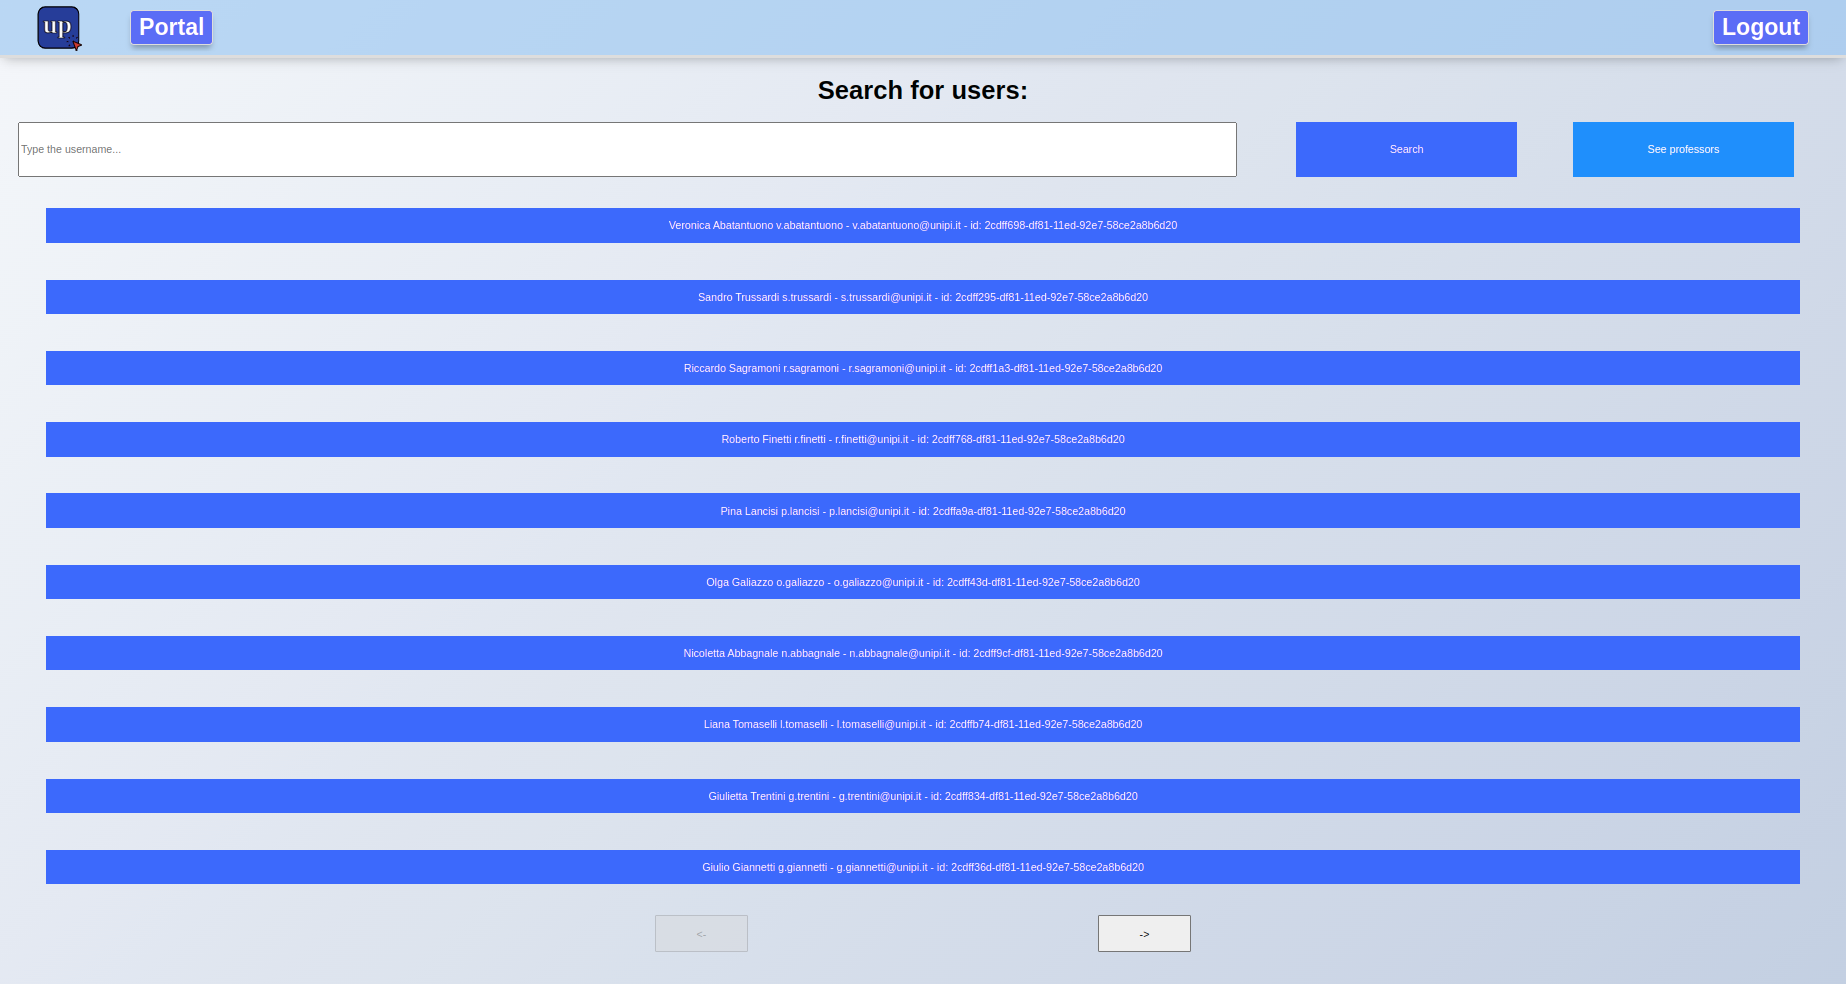
\includegraphics[width=\textwidth]{img/user_manual/admin/admin_search.png}
    \caption{Screenshot of user browsing page}
\end{figure}
After that the admin tried a ban operation an alert will appear to show whether the operation has been successful or not.
\begin{figure}[H]
    \centering
    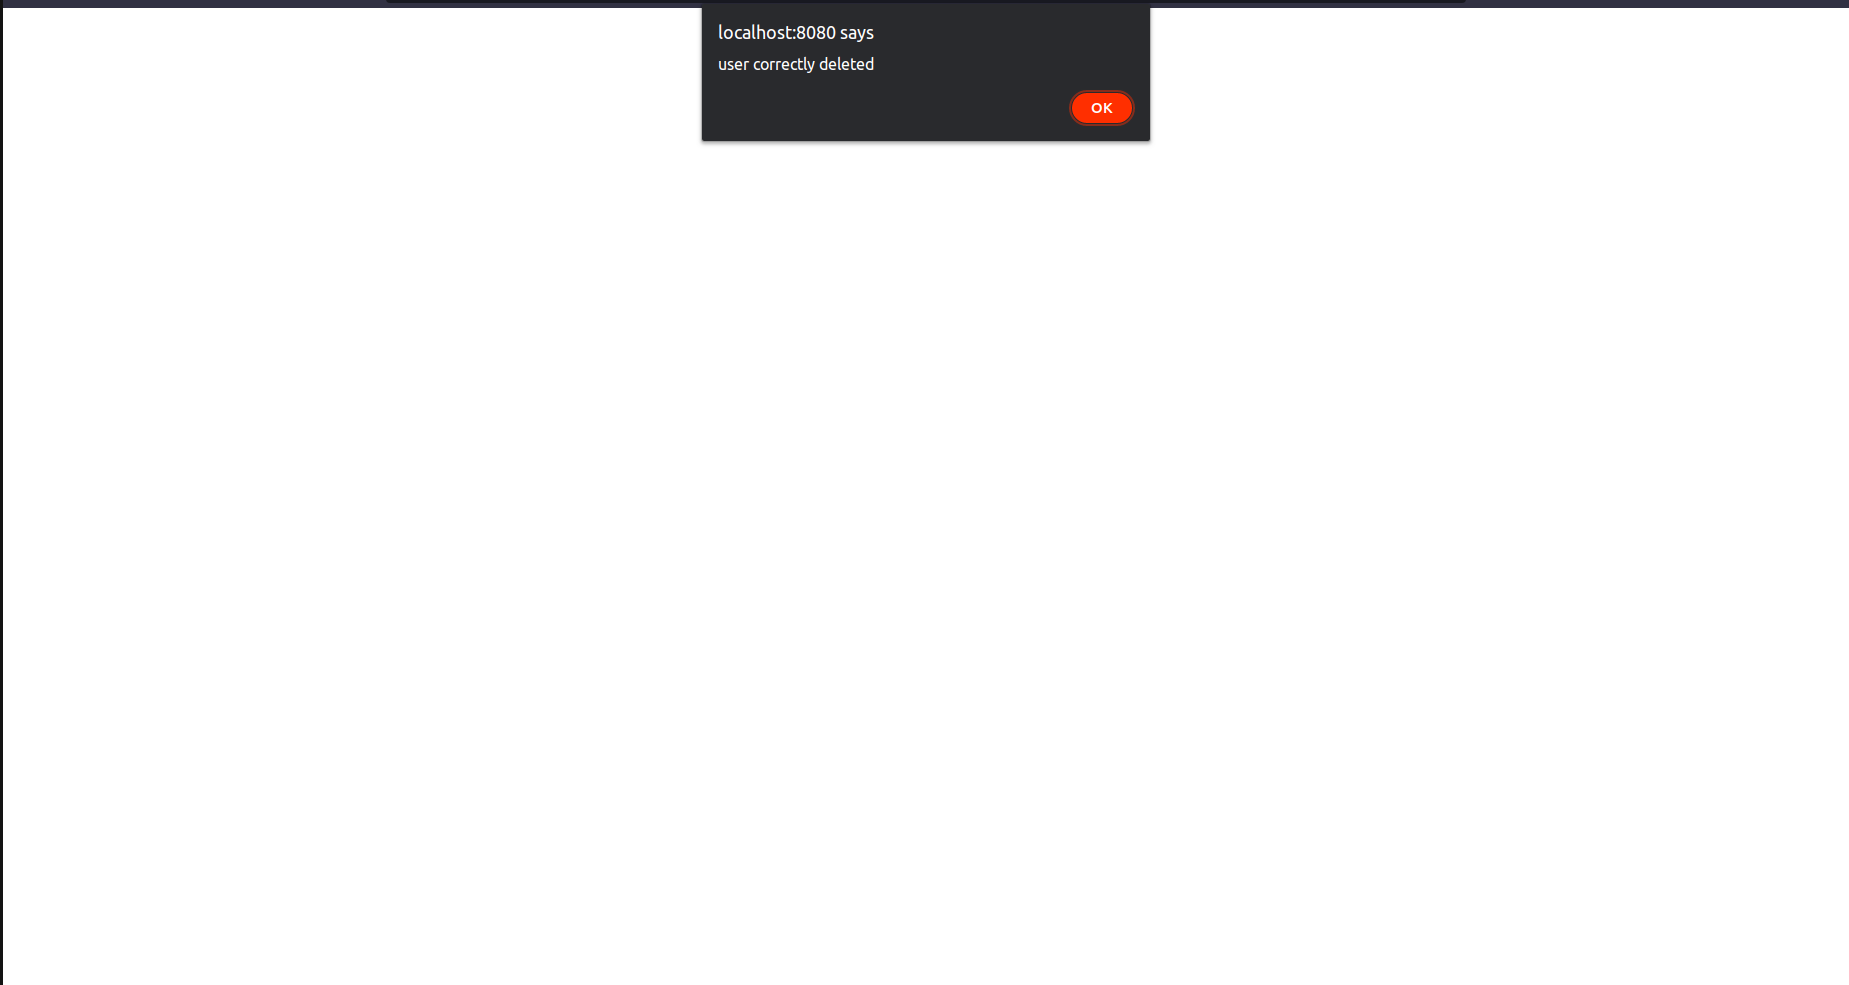
\includegraphics[width=\textwidth]{img/user_manual/admin/ban-response.png}
    \caption{Screenshot of ban response}
\end{figure}